\chapter{Probleembeschrijving}
\label{chap:Probleembeschrijving}
\todo[inline]{nalezen}

Dit hoofdstuk beschrijft het probleem van automatische afbeeldingsbeschrijving. Een eerste sectie gaat over het concrete vraagstuk en hoe het gesitueerd is binnen de computerwetenschappen. Een tweede sectie beschrijft de meest gebruikte datasets voor het trainen en evalueren van systemen die een oplossing bieden voor dit probleem.

\section{Omschrijving en situering}
\label{sec:Omschrijving en situering}
Voor een mens is het beschrijven van een afbeelding zeer eenvoudig. Hij ziet in een oogopslag welke objecten zich op de foto bevinden, en in welke relaties ze zich verhouden. Door een aangeboren taalgevoel is het bedenken van een beschrijvende zin allesbehalve problematisch.
Voor een computer is dit vraagstuk echter veel complexer.

Automatische afbeeldingsbeschrijving bevindt zich op het snijpunt van computervisie en natuurlijke taalverwerking, net door de combinatie van afbeeldingen en tekst. Klassiek gezien worden deze disciplines beschouwd als losstaande vakgebieden. Voor het beschrijven van afbeeldingen is er echter nood aan een combinatie van technieken uit beide vakgebieden. Eerst moeten de verschillende objecten op de foto herkend worden. De computer moet ook een notie hebben van wat elk object net is om daarna een grammaticaal correcte, vloeiende zin te genereren. Om dit laatste te doen is het nodig dat de computer een soort van ``taalgevoel'' heeft. Een ander probleem is de ambigu\"iteit die onvermijdelijk optreedt bij het gebruik van taal en beeld: woorden kunnen verschillende betekenissen hebben, afbeeldingen kunnen op verschillende manieren worden beschreven, \ldots

Het genereren van beschrijvingen is nauw gerelateerd aan andere, eerder onderzochte problemen. Het opzoeken van afbeeldingen is hier het bekendste voorbeeld van. Op basis van een aantal sleutelwoorden, of een volledige zin, wordt een database van afbeeldingen doorzocht naar de afbeelding die het beste overeenkomt met de vraag.

Het automatisch herkennen van objecten in afbeeldingen vormt een van de meest onderzochte vraagstukken in het domein van computervisie. Zoals eerder gezegd, is er niet enkel nood aan algoritmes om vormen te detecteren in afbeeldingen, maar moet er ook een adequate labeling van de gedetecteerde vormen zijn. Een zeer gelijkaardig probleem is het classificeren van een volledige afbeelding, waarbij de hele sc\'ene een label krijgt in plaats van de gedetecteerde objecten. 

De concrete probleemstelling voor het vraagstuk van afbeeldingsbeschrijving is de volgende: ``Genereer een vloeiende, grammaticaal correcte Engelse zin die beschrijft wat er op een nooit eerder geziene foto staat''. Een concreet voorbeeld van twee afbeeldingen met gegenereerde zinnen is te zien in figuur \ref{fig:examplecaptions}.

\begin{figure}[tb]
    \centering
    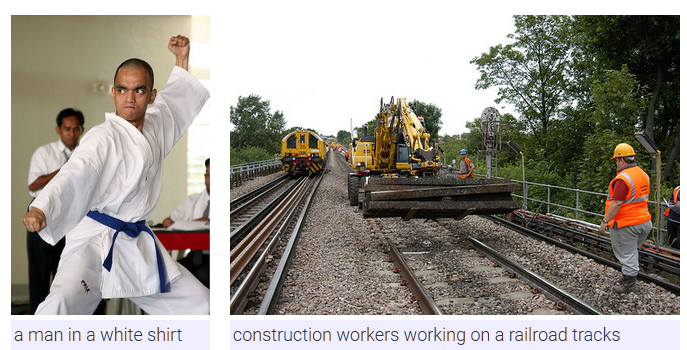
\includegraphics[width= 0.85\linewidth]{Images/caption.PNG}
    \caption{Twee afbeeldingen en hun gegenereerde beschrijving}
    \label{fig:examplecaptions}
\end{figure}

Meer specifiek legt dit proefschrift de focus op het ontwikkelen van een taalmodel dat beter presteert dan een aantal recente systemen. Deze recente systemen vertonen vaak dezelfde gebreken: de gegenereerde zinnen zijn korter dan de zinnen uit de trainingsverzameling, en het aantal unieke woorden ligt vrij laag. Het is de bedoeling van deze masterproef om voor deze gebreken een oplossing te vinden. Dit gebeurt door het toevoegen van extra semantische informatie en het verbeteren van de zoekmethode om zinnen te maken.


\section{Toepassingen}
Het oplossen van dit probleem heeft naast academische ook praktische toepassingen. Zo maakt een dergelijk systeem het mogelijk om voor slechtzienden te beschrijven wat er op de afbeeldingen van een webpagina staat. Daarnaast zijn ook toepassingen denkbaar voor het automatisch ordenen van foto's op basis van dezelfde woorden in de gegenereerde beschrijvingen. Denk maar aan een filter die afbeeldingen filtert met het woord ``sneeuw'' in de beschrijving. Meer algemeen maakt het ook het zoeken naar afbeeldingen op het web eenvoudiger. Zo wordt het mogelijk om naar sleutelwoorden of zinnen te zoeken in de automatisch gegenereerde beschrijvingen. Dit is meer direct dan zoeken op basis van de afbeeldingsnaam, tekst in de omgeving of tags van de afbeelding.


\section{Datasets}
\label{sec:Datasets}
Deze sectie beschrijft de drie meest gebruikte datasets voor training en evaluatie van modellen voor afbeeldingsbeschrijving: Flickr8k, Flickr30k en MS COCO.

\paragraph{Flickr8k}
\label{par:Flickr8k}
De Flickr8k dataset\cite{Hodosh2013}, bevat 8,092 foto's vanop \texttt{flickr.com}. De focus doorheen de afbeeldingen ligt op mensen en dieren (vooral honden) die een actie uitvoeren. De foto's zijn manueel geselecteerd om de grootst mogelijke vari\"eteit te garanderen. De afbeeldingen zijn geselecteerd vanop Flickr\footnote{\url{https://flickr.com}}, een online portaal voor het hosten van afbeeldingen.

De bijhorende beschrijvingen zijn manueel opgesteld door mensen met Engels als moedertaal. De schrijvers maakten gebruik van Amazon Mechanical Turk workers\footnote{\url{http://www.mturk.com}}. Dit is een online platform om ``Human Intelligence Tasks'' te laten uitvoeren door mensen. Tegen een kleine betaling kan iedereen die dat wenst de taken oplossen. 

Een voorafgaande test van de personen die de zinnen schrijven moet de correctheid van de beschrijvingen garanderen. Op basis van een aantal eenvoudige richtlijnen moesten de proefpersonen beschrijvingen voor de afbeeldingen opstellen. De vraag was om objecten en acties te beschrijven in een simpele, maar volledige zin met voldoende adjectieven. Er is geen harde restrictie op het aantal woorden in de beschrijvingen\cite{Hockenmaier2014}.

Eenzelfde afbeelding kan tot verschillende beschrijvingen leiden: sommige mensen focussen op de actie, anderen leggen de nadruk op de persoon die de actie uitvoert, \ldots De zinnen \texttt{A man is skiing down a hill} en \texttt{A man is going down a hill on his skis} beschrijven dezelfde foto, maar doen dit op een verschillende manier. Om deze rijkdom in taal te kunnen weergeven zijn er meerdere zinnen per afbeelding opgenomen in de dataset.

De dataset is verdeeld in drie delen, voor training, validatie en testen. De validatie- en testset bevatten elk 1000 foto's, de trainingsset bevat de overige 6092.


\paragraph{Flickr30k}
\label{par:Flickr30k}
De Flickr30k dataset\cite{Young2014} is een uitbreiding van Flickr8k. Deze uitbreiding is ontstaan vanuit een van de basisprincipes in het machinaal leren: ``Hoe groter de trainingsset, hoe beter het getrainde systeem kan zijn''. In totaal zijn er 31,783 foto's, met elk 5 beschrijvingen. Het proces dat gebruikt is om de dataset op te stellen is hetzelfde als bij Flickr8k. Ook hier bestaan de test- en validatieset uit 1000 foto's, met de resterende 29,783 in de trainingsset.


\paragraph{MS COCO}
\label{par:MS COCO}
De Microsoft Common Objects in COntext dataset (MS COCO)\cite{Lin2014} staat los van de Flickr datasets en probeert een ander type van afbeelding te brengen. Ze bevat meer dan 330,000 afbeeldingen die elk vijf beschrijvingen hebben. 

MS COCO probeert meer te bieden dan ``standaard'' foto's. De auteurs maken een onderscheid tussen afbeeldingen van iconische objecten en iconische sc\`enes, en non-iconische afbeeldingen. Iconische afbeeldingen vormen typisch de eerste zoekresultaten bij een Google Image Search, maar ze bevatten te weinig informatie. Iconische-object afbeeldingen bevatten een centraal geplaatst object. Iconische-scene afbeeldingen bevatten een sc\`ene, meestal zonder aanwezigheid van mensen, vanuit een canonische hoek. Canonische hoeken zijn die aanzichten waarbij de camera quasi loodrecht op de gefotografeerde sc\`ene staat, zij het een boven-, onder-, voor- of zijaanzicht. Hoewel dit type afbeeldingen kan leiden tot zeer goede objectdetecties, is er weinig contextuele informatie aanwezig. Hierdoor zijn beschrijvingen van iconische afbeeldingen minder interessant. Bij de Flickr-datasets is er niet expliciet gefocust op het gebruik van niet-iconische afbeeldingen, dus is er meer vari\"eteit in 

Non-iconische afbeeldingen brengen algemeen gezien een compositie van verschillende objecten en personen, gefotografeerd vanuit een niet-canonische hoek. MS COCO bevat voornamelijk niet-iconische afbeeldingen. Figuur \ref{fig:cocotypes} toont duidelijk het verschil tussen iconische en non-iconische afbeeldingen.

\begin{figure}[tb]
    \centering
    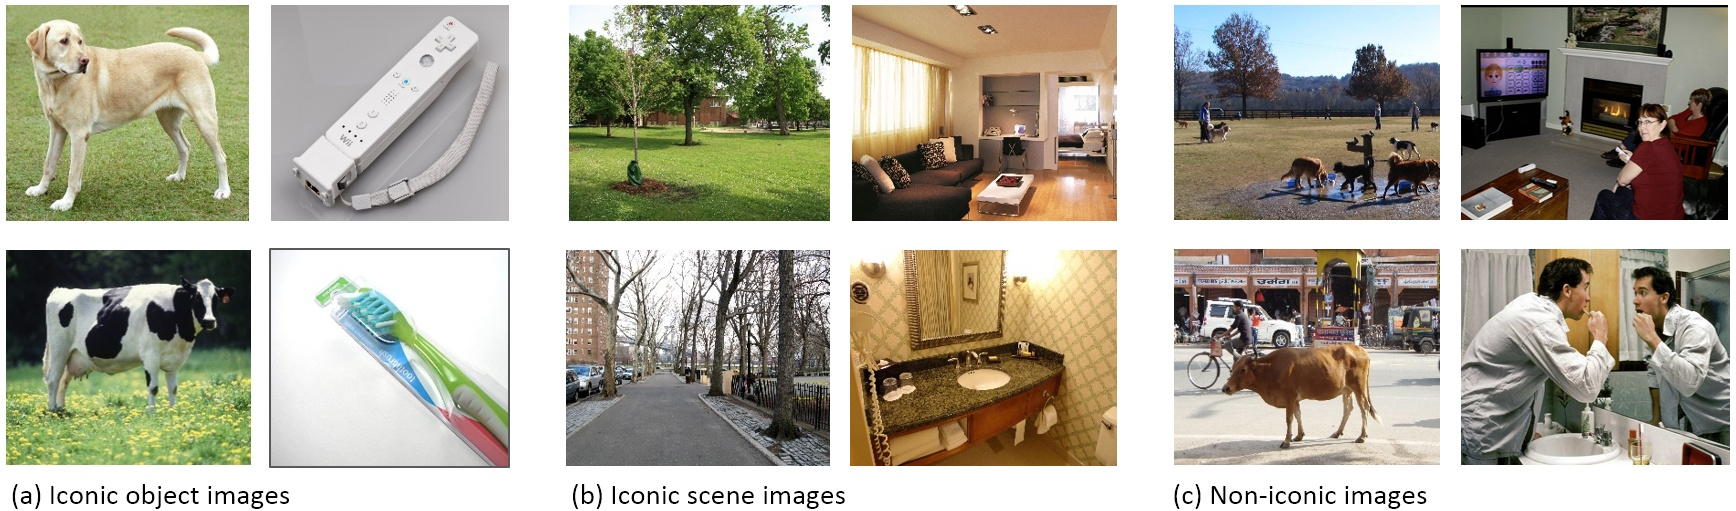
\includegraphics[width=\linewidth]{Images/iconic.jpg}
    \caption{Verschil tussen iconische en non-iconische afbeeldingen}
    \label{fig:cocotypes}
\end{figure}

Een ander belangrijk deel van de COCO dataset zijn annotaties. Oudere datasets legden de focus op classificatie, bounding boxes en segmentatie, terwijl MS COCO probeert om elk belangrijk object op de foto te annoteren. De afbeeldingen zijn gebaseerd op een lijst van object categorie\"en en zijn specifiek geselecteerd om niet-iconische sc\`enes te bevatten.

Het genereren van de beschrijvingen bij de foto's gebeurt met \texttt{Amazon Mechanical Turk workers}, net zoals bij de Flickr datasets. Uitgebreide instructies voor de workers garanderen dat elk belangrijk deel van de afbeelding voorkomt in de beschrijving\cite{Rampf2015}. Figuur \ref{fig:coco_ui} toont op welke wijze de proefpersonen een beschrijving moeten ingeven.


\begin{figure}[tb]
    \centering
    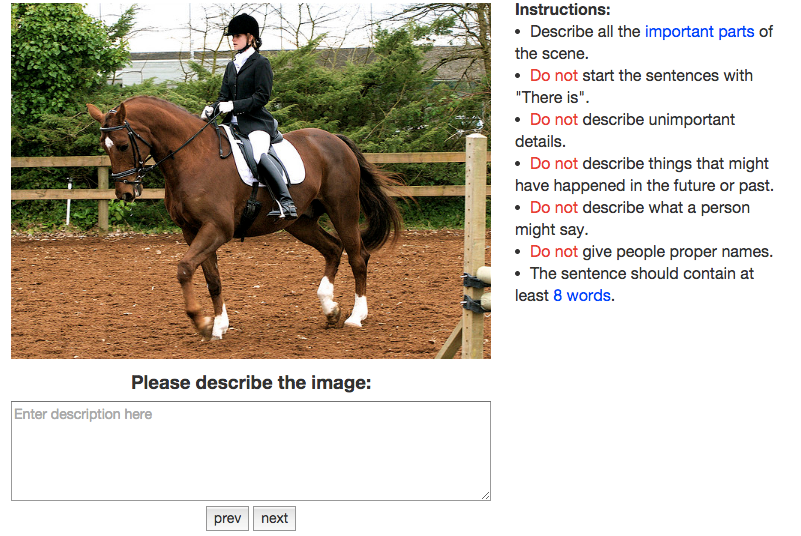
\includegraphics[width=0.8\linewidth]{Images/coco_UI.png}
    \caption{User interface voor het ingeven van afbeeldingsbeschrijvingen MS COCO}
    \label{fig:coco_ui}
\end{figure}

%%% Local Variables: 
%%% mode: latex
%%% TeX-master: "masterproef"
%%% End: 